%package list
\documentclass{article}
\usepackage[top=3cm, bottom=3cm, outer=2cm, inner=2cm]{geometry}
\usepackage{graphicx}
%\usepackage{url}
\usepackage{hyperref}
\usepackage{array}
%\usepackage{multicol}
\newcolumntype{x}[1]{>{\centering\arraybackslash\hspace{0pt}}p{#1}}
%\usepackage{natbib}
%\usepackage{pdfpages}
%\usepackage{multirow}
%\usepackage{float}
%\usepackage[normalem]{ulem}
%\useunder{\uline}{\ul}{}
\usepackage[english,spanish]{babel}
\usepackage[utf8]{inputenc}
\usepackage{fancyhdr}
\usepackage{enumitem}
\usepackage{tikz-qtree}
\usepackage{tikz}
\usetikzlibrary{arrows.meta,bending}
\tikzset{every tree node/.style={minimum width=2.5em,draw,circle},
     blank/.style={draw=none},
     edge from parent/.style=
     {draw, edge from parent path={(\tikzparentnode) -- (\tikzchildnode)}},
     level distance=1.5cm}
\usepackage{minted}
\usetikzlibrary{shapes}

%%%%%%%%%%%%%%%%%%%%%%%%%%%%%%%%%%%%%%%%%%%%%%%%%%%%%%%%%%%%%%%%%%%%%%%%%%%%
%%%%%%%%%%%%%%%%%%%%%%%%%%%%%%%%%%%%%%%%%%%%%%%%%%%%%%%%%%%%%%%%%%%%%%%%%%%%
\newcommand{\csemail}{vmachacaa@unsa.edu.pe}
\newcommand{\csdocente}{Vicente Machaca Arceda}
\newcommand{\cscurso}{Algoritmos y Estructura de Datos}
\newcommand{\csuniversidad}{Universidad Nacional de San Agustín}
\newcommand{\csescuela}{Maestría en Ciencia de la Computación}
\newcommand{\cspracnr}{03}
\newcommand{\cstema}{QuadTree}
%%%%%%%%%%%%%%%%%%%%%%%%%%%%%%%%%%%%%%%%%%%%%%%%%%%%%%%%%%%%%%%%%%%%%%%%%%%%
%%%%%%%%%%%%%%%%%%%%%%%%%%%%%%%%%%%%%%%%%%%%%%%%%%%%%%%%%%%%%%%%%%%%%%%%%%%%


\AtBeginDocument{\selectlanguage{spanish}}
\renewcommand{\figurename}{Figura}
\renewcommand{\refname}{Referencias}
\renewcommand{\tablename}{Tabla}
\AtBeginDocument{%
	\renewcommand\tablename{Tabla}
}

\pagestyle{fancy}
\fancyhf{}
\setlength{\headheight}{30pt}
\renewcommand{\headrulewidth}{1pt}
\renewcommand{\footrulewidth}{1pt}
\fancyhead[L]{\raisebox{-0.2\height}{
\includegraphics[width=3cm]{img/logo_unsa}}}
\fancyhead[C]{}
\fancyhead[R]{\fontsize{7}{7}\selectfont	\csuniversidad \\ \csescuela \\ \textbf{\cscurso} }
\fancyfoot[L]{MSc. Vicente Machaca}
\fancyfoot[C]{\cscurso}
\fancyfoot[R]{Página \thepage}

%\usemintedstyle{vs}

\begin{document}
	
	\vspace*{10px}
	
	\begin{center}	
		\fontsize{17}{17} \textbf{ Práctica \cspracnr}
	\end{center}

	\begin{table}[h]
		\begin{tabular}{|x{5.4cm}|x{5.4cm}|x{5.4cm}|}
			\hline 
			\textbf{DOCENTE} & \textbf{CARRERA}  & \textbf{CURSO}   \\
			\hline 
			\csdocente & \csescuela & \cscurso    \\
			\hline 
		\end{tabular}
	\end{table}	
	
	\begin{table}[h]
		\begin{tabular}{|x{5.4cm}|x{5.4cm}|x{5.4cm}|}
			\hline 
			\textbf{PRÁCTICA} & \textbf{TEMA}  & \textbf{DURACIÓN}   \\
			\hline 
			\cspracnr & \cstema & 3 horas   \\
			\hline 
		\end{tabular}
	\end{table}
	
	\section{Datos de los estudiantes}
	\begin{enumerate}
		\item \textbf{Grupo:} 09
		\item \textbf{Integrantes:}
		\begin{itemize}
			\item Asmat Fuentes, Franz Rogger
			\item Esthela Espinoza, Fausto Danilo
			\item Ojeda Mamani, Abel Eberth
			\item Paredes Rodriguez, Raybert
		\end{itemize}		
	\end{enumerate}
	
	\section{Ejercicios}\label{sec:ejercicios}
	\begin{enumerate}
        
        \item {Cree un archivo \textit{main.html}, este invocará a los archivos Javascript que vamos a crear. El archivo \textit{p5.min.js} es una librería para gráficos, la puede descargar de internet o se la puede pedir al profesor. En el archivo \textit{quadtree.js} estará todo el código de la estructura y en el archivo \textit{sketch.js} estará el código donde haremos pruebas del Quadtree.}

            \begin{minted}
            [
                frame = lines,
                framesep = 2mm,
                obeytabs = true,
                tabsize = 2
            ]
            {html} 
            <html>
            
            <head>
                <title> QuadTree </title>
                <script src="scripts/p5.min.js"> </script>
                <script src="scripts/quadtree.js"> </script>
                <script src="scripts/sketch.js"> </script>

                <style>
                    body{
                        font-family: Ubuntu, Arial, sans-serif;
                    }
                    .grid-container {
                        display: grid;
                        grid-template-columns: auto auto auto;
                        padding: 5px;
                    }
                    .grid-container>div {
                        text-align: center;
                        padding: 5px;
                    }
                </style>
            </head>
            
            <body>
                <div class="grid-container">
            		<div class="grid-item" style="vertical-align: middle;">
            			<img id="logoUnsa" src="img/logo_unsa.jpg" width="200" alt="UNSA">
            		</div>
            		<div class="grid-item">
            			<p style="font-size: 18px;font-weight: bold;">
            				Universidad Nacional de San Agust&iacute;n<br />
            				Maestr&iacute;a en Ciencias de la Computaci&oacute;n<br />
            				Algoritmos y Estructura de Datos<br />
            			</p>
            		</div>
            		<div class="grid-item">
            			<p style="font-size: 18px;font-weight: bold;">
                            Pr&aacute;ctica 03
            			</p>
                    </div>
            		<div class="grid-item">&nbsp;</div>
            		<div class="grid-item"><div id="QuadTreeCanvas"></div></div>
            		<div class="grid-item">&nbsp;</div>
            	</div>
            </body>
            </html>
            \end{minted}            

        
        \item En el archivo \textit{quadtree.js} digitemos el siguiente código, además debe completar las funciones \textit{contains} e \textit{intersects} (ambas funciones devuelven \textit{true} o \textit{false}).
        
            \begin{minted}
            [
                frame = lines,
                framesep = 2mm,
                obeytabs = true,
                tabsize = 2
            ] {javascript}
            
            contains(point) {
                return (point.x >= this.x - this.w && 
                        point.x <= this.x + this.w && 
                        point.y >= this.y - this.h && 
                        point.y <= this.y + this.h );
            }
            
            intersects(range) {
                return !(range.x - range.w > this.x + this.w || 
                         range.x + range.w < this.x - this.w || 
                         range.y - range.h > this.y + this.h || 
                         range.y + range.h < this.y - this.h);
            }
            
            \end{minted}
        
        \item En el archivo \textit{quadtree.js} digitemos el siguiente código y complete las funciones \textit{subdivide} e \textit{insert}.
        
         \begin{minted}
            [
                frame = lines,
                framesep = 2mm,
                obeytabs = true,
                tabsize = 2
            ] {javascript}

            subdivide() {
                let x = this.boundary.x;
                let y = this.boundary.y;
                let w = this.boundary.w;
                let h = this.boundary.h;
                let qt_northeast = new Rectangle(x + w / 2, y - h / 2, w / 2, h / 2);
                let qt_northwest = new Rectangle(x - w / 2, y - h / 2, w / 2, h / 2);
                let qt_southeast = new Rectangle(x + w / 2, y + h / 2, w / 2, h / 2);
                let qt_southwest = new Rectangle(x - w / 2, y + h / 2, w / 2, h / 2);
                this.northeast = new QuadTree(qt_northeast, this.capacity);
                this.northwest = new QuadTree(qt_northwest, this.capacity);
                this.southeast = new QuadTree(qt_southeast, this.capacity);
                this.southwest = new QuadTree(qt_southwest, this.capacity);
                this.divided = true;
            }

            insert(point) {
                if (!this.boundary.contains(point)){
                    return false;
                }
        
                if (this.points.length < this.capacity) {
                    this.points.push(point);
                    return true;
                } 
                else {
                    if(!this.divided){                
                        this.subdivide();                
                    }
                    return (
                        this.northeast.insert(point) ||
                        this.northwest.insert(point) ||
                        this.southeast.insert(point) ||
                        this.southwest.insert(point)
                      );
                }
            }
         \end{minted}
        
        \item {Editemos el archivo \textit{sketch.js}. En este archivo estamos creando un QuadTree de tamaño 400x400 con 3 puntos. Ejecute (obentrá un resultado similar a la Figura 1)}
        
        \begin{minted}
            [
                frame = lines,
                framesep = 2mm,
                obeytabs = true,
                tabsize = 2
            ] {javascript}
            
            function setup() {
                let quadCanvas = createCanvas(400, 400);
                quadCanvas.parent("QuadTreeCanvas");
                let boundary = new Rectangle(200, 200, 200, 200);
                qt = new QuadTree(boundary, 4);
            
                console.log(qt);
                for (let i = 0; i < 3; i++) {
                    let p = new Point(Math.random() * 400, Math.random() * 400);
                    qt.insert(p);
                }
            
                background(0);
                qt.show();
            }
            
        \end{minted}
        \begin{center}
            \frame{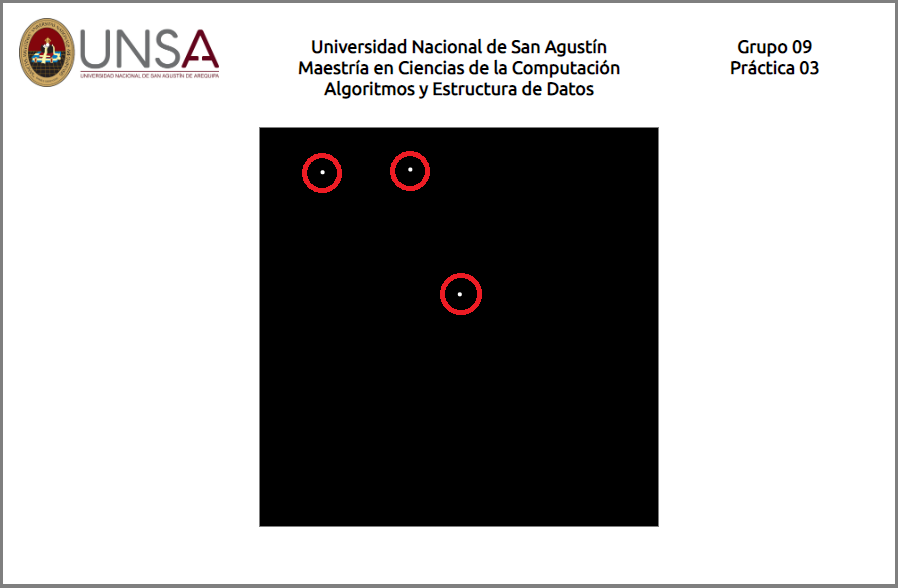
\includegraphics[width=15cm]{img/Figura_01}}\par
            \textit{Figura 1: Resultado de insertar tres (3) puntos}
        \end{center}
        
        \item {Abra las opciones de desarrollador (opciones / más herramientas / opciones de desarrollador) de su navegador para visualizar la console (Figura 2).}
        
        
        \begin{center}
            \frame{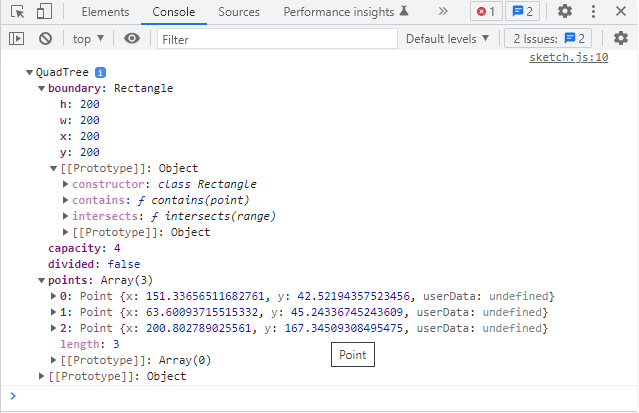
\includegraphics[width=13cm]{img/Figura_02}}\par
            \textit{Figura 2: Visualización de herramientas de desarrollo}
        \end{center}
        
        \item {Edite el archivo \textit{sketch.js} con el siguiente código. En este caso, nos da la posibilidad de insertar los puntos con el mouse.}
        
        \begin{minted}
            [
                frame = lines,
                framesep = 2mm,
                obeytabs = true,
                tabsize = 2
            ] {javascript}
        
        function draw() {
            background(0);
            if (mouseIsPressed) {
                for (let i = 0; i < 1; i++) {
                    let m = new Point(mouseX + random(-5, 5), mouseY + random(-5,5));
                    console.log(m);
                    qt.insert(m);
                }
            }
            qt.show();
        }
        
        \end{minted}
        
        \begin{center}
            \frame{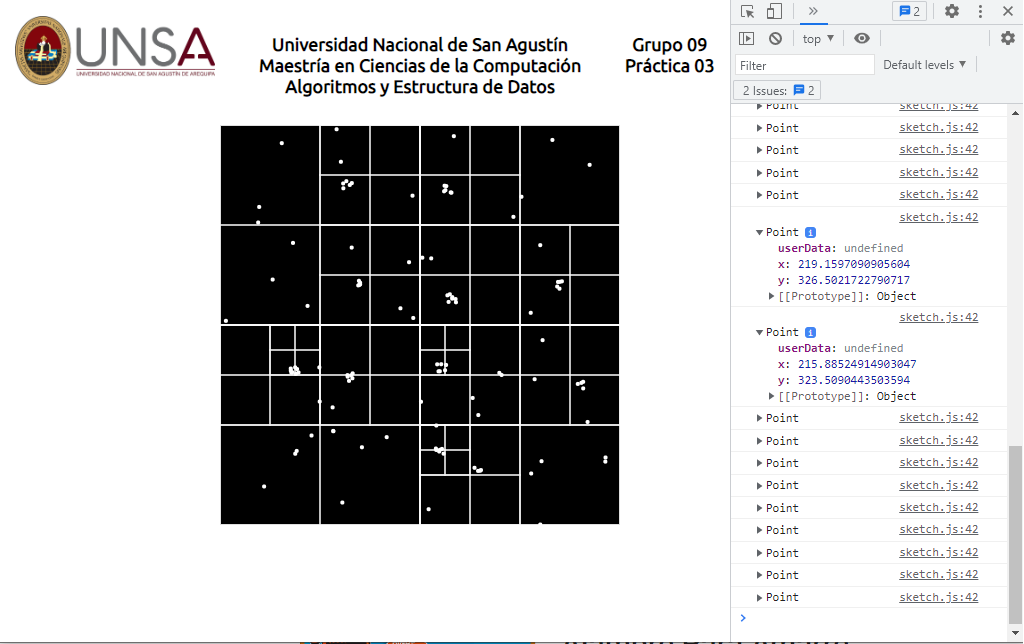
\includegraphics[width=15cm]{img/Figura_03}}\par
            \textit{Figura 3: Quadtree, inserción de puntos con mouse}
        \end{center}


        \item {Edite el archivo \textit{quadtree.js} y complete la función query.}
        
        \begin{minted}
        [
            frame = lines,
            framesep = 2mm,
            obeytabs = true,
            tabsize = 2
        ] {javascript}
        
        query(range, found){    
            if(!found){
                found=[];
            }
            if(!this.boundary.intersects(range)){
                return found;
            }
            else{
              for(let point of this.points){
                if(range.contains(point)){
                    found.push(point)
                }
              }
              if(this.divided){            
                this.northeast.query(range,found);
                this.northwest.query(range,found);
                this.southeast.query(range,found);
                this.southwest.query(range,found);
              } 
              return found;
            }
        }
        \end{minted}   
        
        \item {Editemos el archivo \textit{sketch.js}, En este caso haremos consultas con el mouse}
        
        \begin{minted}
        [
            frame = lines,
            framesep = 2mm,
            obeytabs = true,
            tabsize = 2
        ] {javascript}
        
        let qt;
        let count = 0;
        
        function setup () {
            createCanvas (400 ,400);
            let boundary = new Rectangle (200, 200, 200, 200);
            qt = new QuadTree (boundary , 4);
            
            console.log (qt);
            for (let i=0; i < 25; i ++) {
                let p = new Point (Math.random () * 400 , Math.random () * 400);
                qt.insert (p);
            }
            background (0);
            qt.show ();
        }
        
        function draw () {
            background (0);
            qt.show ();
            
            stroke (0 ,255 ,0);
            rectMode (CENTER);
            let range = new Rectangle (mouseX, mouseY, 50, 50);
            rect (range.x, range.y, range.w * 2, range.h * 2);
            let points = [];
            qt.query (range, points);
            
            for (let p of points) {
                strokeWeight (4);
                point (p.x, p.y);
            }
        }
        \end{minted}  
        
        \par
	    \begin{center}
	        \url{https://unsa-mcc-2022.github.io/AyED_Practica_03/index.html}
	    \end{center}
        
        \begin{center}
            \frame{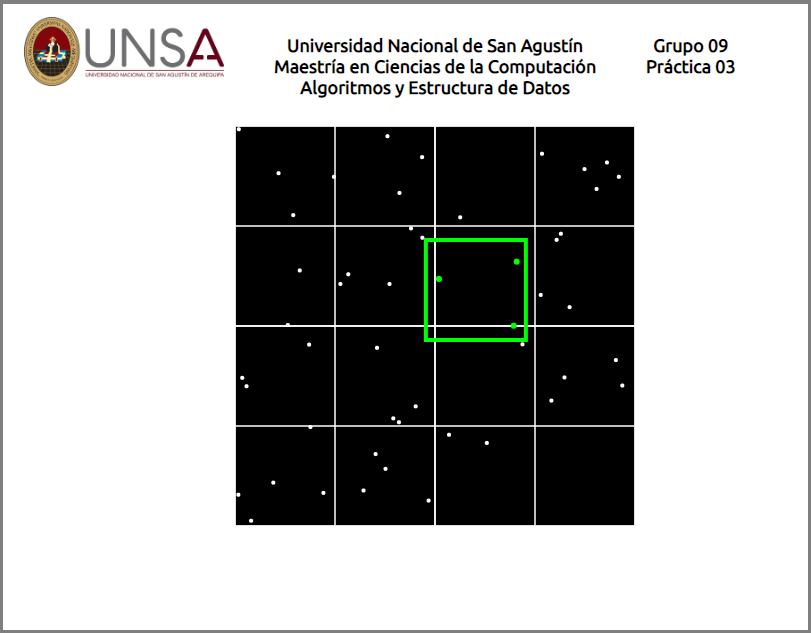
\includegraphics[width=15cm]{img/Figura_04}}\par
            \textit{Figura 4: Implementación de búsqueda (Query)}
        \end{center}
        
        
        \item {Finalmente, debe implementar un \textit{Octree} y visualizarlo. Puede utilizar cualquier lenguaje de programación.}
        
        \begin{center}
        \textbf{Ejemplo en funcionamiento}
        \end{center}
        
        \par
	    \begin{center}
	        \url{https://unsa-mcc-2022.github.io/AyED_Practica_03/octree.html}
	    \end{center}
        
        
        \begin{center}
            \frame{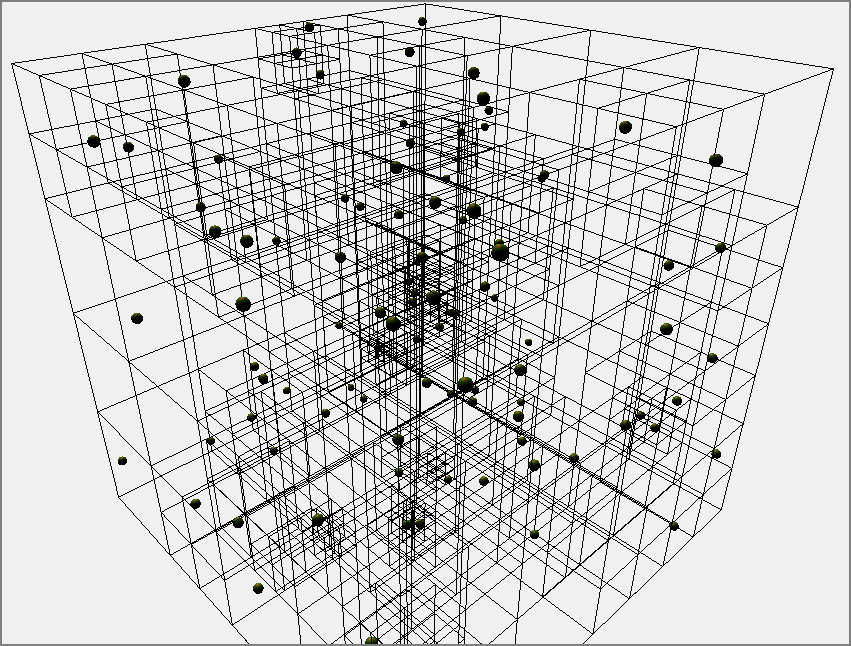
\includegraphics[width=15cm]{img/Figura_05}}\par
            \textit{Figura 5: Octree en funcionamiento}
        \end{center}
        
        \begin{center}
            \textbf{Código fuente (Javascript)}
        \end{center}
        
        \begin{minted}
        [
            frame = lines,
            framesep = 2mm,
            obeytabs = true,
            tabsize = 2
        ] {javascript}

 function Octree(parent, origin, halfwidth, halfheight, halfdepth) {
	this.origin = origin;
	this.halfwidth = halfwidth;
	this.halfheight = halfheight;
	this.halfdepth = halfdepth;

	this.depth = parent === null ? 0 : parent.depth + 1;

	this.entities = new Array();	

	this.parent_node = parent;
	this.children_nodes = new Array();

	this._all_entities = new Array();	// {entity, node}, TODO: verifique si hay una manera de convertirlo en una entidad de mapa-> nodo
	this._to_update = parent === null ? new Array() : parent._to_update;
	this._leaves = new Array();
	this._leaves.push(this);

	this._need_leaves_update = false;
	this._need_all_entities_update = false;

	var _this = this;

	this.onEntityPoseChanged = function(entity) {
		if(_this._to_update.indexOf(entity) === -1)
			_this._to_update.push(entity);
	}

	// representación visual con fines de depuración
	var geo = new THREE.CubeGeometry( halfwidth*2, halfheight*2, halfdepth*2 );
	
	this.mesh = new THREE.Mesh( geo, new THREE.MeshBasicMaterial( { color: 0x0, opacity: 1, wireframe: true } ) );
	this.mesh.position = origin.clone();

	if(parent !== null)
	{
		this.mesh.position.sub(parent.origin);
		parent.mesh.add(this.mesh);
	}
	//
}

Octree.prototype.constructor = Octree;

Octree.prototype.entities_per_node = 1;
Octree.prototype.max_depth = 5;

Octree.prototype.add = function(entity) {

	var _this = this;
	function addToThis() {
		var iter = _this;
		while(iter !== null)
		{
			iter._need_all_entities_update = true;
			iter = iter.parent_node;
		}
		_this.entities.push(entity);
		_this.mesh.visible = true;
	}

	if(!this.intersects(entity))
		return;

	if(this.depth >= this.max_depth)
	{
		addToThis();
	}
	else if(this.children_nodes.length == 0)
	{
		if(this.entities.length < this.entities_per_node)
		{
			addToThis();
		}	
		else
		{	
			this.subdivide();

			if( this.entities.length !== 0 ) 
			{
				var entities_tmp = this.entities.slice();
				this.entities.length = 0;
				while(entities_tmp.length > 0)
				{
					var ent = entities_tmp.pop();
					this.remove(ent);
					this.add(ent);
				}
			}

			this.add(entity);
		}
			
	}
	else
	{
		// verificar si el obb se cruza (intersects) con varios hijos
		var child_id = -1;
		var multiple_intersect = false;
		for(var i = 0; i < this.children_nodes.length; i++)
		{
			if(this.children_nodes[i].intersects(entity))
			{
				if(child_id != -1)
				{
					multiple_intersect = true;
					break;
				}
				child_id = i;
			}
		}

		if(multiple_intersect)
		{
			addToThis();
		}
		else
			this.children_nodes[child_id].add(entity);
	}
};

Octree.prototype.remove = function(entity) {
	for(var i = 0; i < this.entities.length; i++ )
	{
		if(this.entities[i] === entity)
		{
			this.entities.splice(i, 1);
			break;
		}		
	}

	var iter = this;
	while(iter !== null)
	{
		iter._need_all_entities_update = true;
		iter = iter.parent_node;
	}
};

Octree.prototype.empty = function(){
	if(this.entities.length > 0)
		return false;

	for(var i = 0; i < this.children_nodes.length; i++)
	{
		if(!this.children_nodes[i].empty())
			return false;
	}
	return true;
};

Octree.prototype.intersects = function(entity) {
	return this.contains(entity.position);
};

Octree.prototype.contains = function(point) {
	var diff = new THREE.Vector3();
	diff.subVectors( point, this.origin );

	return Math.abs(diff.x) <= this.halfwidth && Math.abs(diff.y) <= this.halfheight && Math.abs(diff.z) <= this.halfdepth;
};

Octree.prototype.subdivide = function() {

	/*       _____________
		   /  4   /  5   /|        y
		  /_____ /______/ |        |
	     /      /      /| |        |___ x
		/_____ / _____/ |/|       / 
		|   0  |  1   | |7|      /
		|_____ |_____ |/|/       z
		|   2  |  3   | /
		|_____ |_____ |/ (lol)
	*/

	if(this.depth >= this.max_depth)
		return;

	this.needLeavesUpdate();

	var qwidth = this.halfwidth / 2;
	var qheight = this.halfheight / 2;
	var qdepth = this.halfdepth / 2;

	this.children_nodes[0] = new Octree( this, new THREE.Vector3( this.origin.x - qwidth, 
													  this.origin.y + qheight, 
													  this.origin.z + qdepth ),
								   qwidth, qheight, qdepth);

	this.children_nodes[1] = new Octree( this, new THREE.Vector3( this.origin.x + qwidth, 
													  this.origin.y + qheight, 
													  this.origin.z + qdepth ),
								   qwidth, qheight, qdepth);

	this.children_nodes[2] = new Octree( this, new THREE.Vector3( this.origin.x - qwidth, 
													  this.origin.y - qheight, 
													  this.origin.z + qdepth ),
								   qwidth, qheight, qdepth);

	this.children_nodes[3] = new Octree( this, new THREE.Vector3( this.origin.x + qwidth, 
													  this.origin.y - qheight, 
													  this.origin.z + qdepth ),
								   qwidth, qheight, qdepth);

	this.children_nodes[4] = new Octree( this, new THREE.Vector3( this.origin.x - qwidth, 
													  this.origin.y + qheight, 
													  this.origin.z - qdepth ),
								   qwidth, qheight, qdepth);

	this.children_nodes[5] = new Octree( this, new THREE.Vector3( this.origin.x + qwidth, 
													  this.origin.y + qheight, 
													  this.origin.z - qdepth ),
								   qwidth, qheight, qdepth);

	this.children_nodes[6] = new Octree( this, new THREE.Vector3( this.origin.x - qwidth, 
													  this.origin.y - qheight, 
													  this.origin.z - qdepth ),
								   qwidth, qheight, qdepth);

	this.children_nodes[7] = new Octree( this, new THREE.Vector3( this.origin.x + qwidth, 
													  this.origin.y - qheight, 
													  this.origin.z - qdepth ),
								   qwidth, qheight, qdepth);
};

// conteo de la máxima intersección de hijos.
Octree.prototype.countChildrenIntersections = function(max, entity) {
	var children_idx = new Array();
	for(var j = 0; j < this.children_nodes.length; j++)
	{
		if(this.children_nodes[j].intersects(entity))
			children_idx.push(j);
		if(children_idx.length === max)
			break;
	}
	return children_idx;
}

Octree.prototype.needLeavesUpdate = function() {
	var iter = this;
	while(iter !== null)
	{
		iter._need_leaves_update = true;
		iter = iter.parent_node;
	}
}

// actualiza la referencia de las entidades hijas 
Octree.prototype.updateChildrenEntities = function() {
	if(this._need_all_entities_update)
	{
		this._all_entities.length = 0;
		for(var i = 0; i < this.children_nodes.length; i++)
		{
			this.children_nodes[i].updateChildrenEntities();
			this._all_entities = this._all_entities.concat(this.children_nodes[i]._all_entities);
		}

		for(var i = 0; i < this.entities.length; i++)
		{
			this._all_entities.push([this.entities[i], this]);
		}
	}
}

// actualiza los hojas (leaves) de referencia
Octree.prototype.updateLeaves = function() {
	if(this._need_leaves_update)
	{
		this._leaves.length = 0;
		for(var i = 0; i < this.children_nodes.length; i++)
		{
			
			this.children_nodes[i].updateLeaves();
			this._leaves = this._leaves.concat(this.children_nodes[i]._leaves);
		}

		if(this.children_nodes.length === 0)
			this._leaves.push(this);

		this._need_leaves_update = false;
	}
}

Octree.prototype.update = function() {

	var _this = this;
	_this.updateChildrenEntities();
	var entities_tmp = this._all_entities.slice();
	entities_tmp.forEach( function(element) {
		var entity = element[0];
		
		for(var i = 0; i < _this._to_update.length; i++)
		{
			if( entity === _this._to_update[i] )
			{
				var octree;
				var intersections;

                // comprueba si hay intersección múltiple con hijos
                // si es así, haga lo mismo recursivamente con los padres hasta que podamos ajustarlo por completo
                // en un nodo y agregarlo a este nodo
				octree = element[1];
				while(octree !== null)
				{
					intersections = octree.countChildrenIntersections(2, entity);
					
					if(intersections.length === 1)
					{
						// no realice ninguna operación si no se requiere ninguna actualización
						if(element[1] === octree.children_nodes[intersections[0]])
							break;
						element[1].remove(entity);
						octree.children_nodes[intersections[0]].add(entity);
						break;
					}
					else if(octree.parent_node === null && intersections.length > 0) 
					{
						element[1].remove(entity);
						octree.add(entity);
						break;
					}
					else
						octree = octree.parent_node;
				}
				_this._to_update.splice(i,1);
				break;
			}
		}
	});

	// actualiza todas las matrices _all_entities
	_this.updateChildrenEntities();
 
	_this.updateLeaves();

	function pruneUp(node) {
		if(node._all_entities.length <= 1)
		{			
            // remueve a los hijos de la matriz(leaves) y separe su malla de los padres
			(function removeChildrenNodes(node) {
				for(var i = 0; i < node.children_nodes.length; i++)
				{
					removeChildrenNodes(node.children_nodes[i]);
					var idx = _this._leaves.indexOf(node.children_nodes[i]);
					if( idx !== -1 )
						_this._leaves.splice(idx, 1);
					node.mesh.remove(node.children_nodes[i].mesh);
				}
			})(node);

			node.needLeavesUpdate();
			node.children_nodes.length = 0;

			if(node._all_entities.length === 1 && (node._all_entities[0])[1] !== node)
			{
				// if the entity was in a one of the child, put it in current node
                //si la entidad estuvo en uno de los hijos, colocarlo en el nodo actual
				node._all_entities[0][1] = node;	// actualizará esta referencia para el nodo de los padres también
				node.add(node._all_entities[0][0]);
			}
			if(node.parent_node !== null)
			{
				pruneUp(node.parent_node);
			}	
		}
	}

	this._leaves.forEach( function(node){
		pruneUp(node);
	});	
};

        \end{minted}  

    \end{enumerate}
    
    \section{Repositorio}\label{sec:codigo}
        La implementación de los algoritmos y los datos utilizados es el siguiente:\par
	    \par
	    \begin{center}
	        \url{https://github.com/UNSA-MCC-2022/AyED_Practica_03}
	    \end{center}

    \section{Representación gráfica}\label{sec:representacion}
        Se realizó la implementación de la representación gráfica de los algoritmos indicados, esto se pueden visualizar en el siguiente enlace:\par
	    \par
	    \begin{center}
	        \url{https://unsa-mcc-2022.github.io/AyED_Practica_03}
	    \end{center}
	
	%\clearpage
	%\bibliographystyle{apalike}
	%\bibliographystyle{IEEEtranN}
	%\bibliography{bibliography}
		
	
\end{document}